\section{Introduction}
\par The importance of quality calibration for this work is mainly justified by skepticism towards the camera's factory calibration and the quality of the used software. Because the camera's software presents big constraints and brings large sources of mistakes with unknown origins, the best way to process the results is to obtain the RAW data and treat it resorting to a special made Matlab code and a blackbody calibration. \\
\section{Blackbody Calibration Sources}
\par Black Body Calibration sources are recommended by the camera manual to calibrate the camera correctly. They are simply blackbodies with controllable temperature. The temperature controlled blackbody is to be filmed by the IR Camera and the camera's raw data (signal intensity received by the sensors) extracted. With a known temperature and high emissivity it is easy to correlate the signal intensity with the correspondent temperature. Establishing this relation can be done directly in the software but for the reasons referred in the previous section it was done with matlab and excel.\\

\par The Blackbody Calibration Source is the name given to these devices, that are commercialized to calibrate infrared sensors. Because the price of the simplest one can be over 7000 euros, it was decided that one should be created, having in mind the principles of these devices. \\

\par There are several types of blackbody calibration sources, which are included in these main categories \cite{blackbody}: 
\begin{itemize}
\item Fixed-Point Blackbody Radiators: used at really high temperatures (>1000ºC), these are characterized by having a metal (eg. Au, Ag or Cu) at freezing point and a graphite made cavity (high emissivity). The quality of the measure is defined by the quality of the graphite, metal ingot and shape of the cavity.
\item Heat Pipe Cavities: used at temperatures from -60ºC to 1000ºC, depending on the work fluid, these are characterized by having the best precision, and being the most sophisticated devices. They work by having the cavity surrounded by a multistate heated fluid at a controlled pressure. This cavity has special geometric properties to enhance the emissivity of the body. They are usually used in high precision applications like meteorology institutes.
\item Pratical Cavities: used in more pratical applications, their temperature range goes from -45ºC to 450ºC. Unlike the Heat Pipe, the working fluid rarely changes its physical state (eg. one could only go up until 100ºC with water). Pratical cavities have a simpler build and are often used for testing by the radiation thermometers manufacturers. As the latter, Pratical Cavities also rely on specific geometric conditions to enhance the cavity's emissivity.
\item Flat Plate: these devices are used as an alternative to the devices above because they do not require small cavities. With this in mind its obvious the counterpart of this type. The heated plate needs a high emissivity paint and it generates bigger uncertainties. This method is usually used for bigger applications.
\item Others: Cryogenic/Vaccum Blacbodies, used in low temperatures and Furnaces, used as Flat Plate for applications above 1000ºC.
\end{itemize}

\par For this work, the Pratical Cavity Radiator is the best choice, not only because it's often used in the same applications and temperature range but also because it is the simplest solution to produce. The final design of the chamber was based on the scheme presented in Hartmann's work \cite{blackbody}, and it's presented in Figure \ref{fig:bbs} and the cavity shape based on the design proposed in Figure \ref{fig:blkbody}. Because the camera had to be calibrated to work between the temperatures of 0 and 130ºC, the working fluid had to be oil, because of its higher saturation temperature. \\

\begin{figure}
\centering
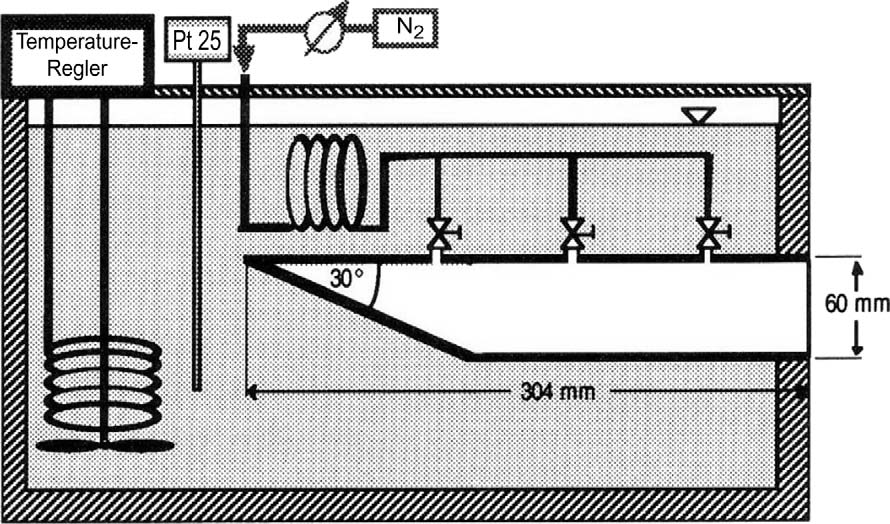
\includegraphics[width=0.6\linewidth]{Figures/4.Chapter/praticalcavity.png}
\caption{Pratical Cavity Blackbody Source scheme}
\source{Chapter 3.2 from \cite{blackbody}}
\label{fig:bbs}
\end{figure}


\par The effect demonstrated in Figure \ref{fig:blkbody} is used in many cavity based Blackbody Radiator Devices and serves to enhance the emissivity, by trapping the light, thus reducing light reflected from the outside. This effect is enhanced by an angle of 30º as referenced in the literature \cite{blackbody}. A working scheme for the final design of the created device, with a mixture of these 2 concepts is presented in Figure \ref{fig:box}. \\

\begin{figure}[h]
\centering
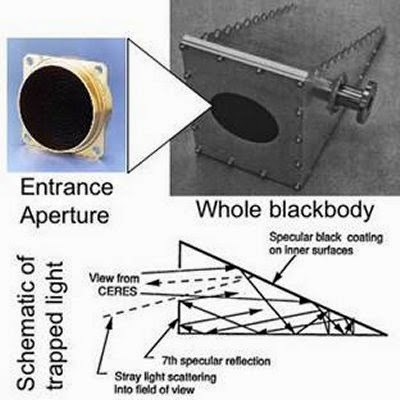
\includegraphics[width=0.6\linewidth]{Figures/4.Chapter/blackbody3.jpg}
\caption{Cavity and light trapping effect scheme}
\source{NASA}
\label{fig:blkbody}
\end{figure}

\begin{figure}[h]
\centering
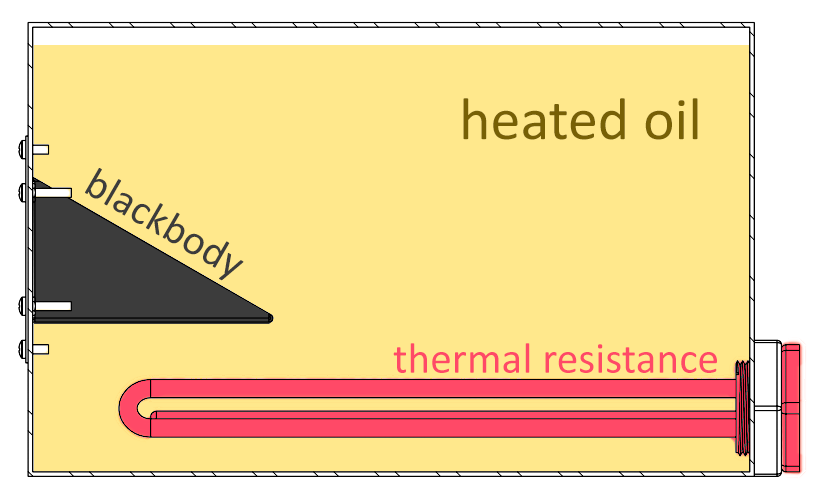
\includegraphics[width=0.6\linewidth]{Figures/4.Chapter/caixa.png}
\caption{Final design scheme for the Blackbody Calibration Source}
\label{fig:box}
\end{figure}

\subsection{Design details}
\par The final design render, made in SolidWorks, can be seen in Figure \ref{fig:render}. One may notice, both from the render and the scheme, that the box is too long compared to the blackbody. The reason for this is that the whole machine had to be made to fit the only available thermal resistance in the store. This resistance is presented in Figure \ref{fig:res}. The working fluid has to be durable and have good conductive properties, so the type of oil used was car oil, due to its durability and thermal properties. \\

\begin{figure}[h]
\centering
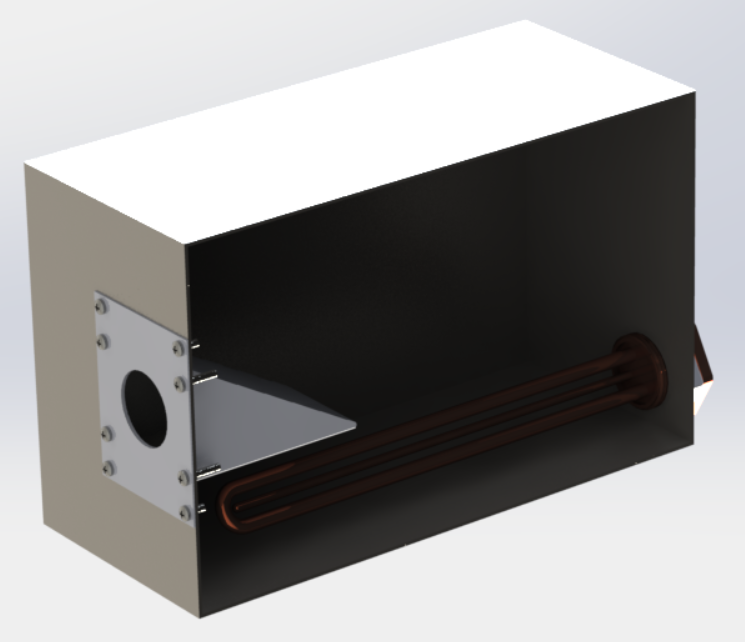
\includegraphics[width=0.8\linewidth]{Figures/4.Chapter/caixa_render.PNG}
\caption{SolidWorks render of a cut device view}
\label{fig:render}
\end{figure}

\par In both the scheme and render, the sensors, peripherals of the machine and its insulation are omitted. In this machine 5 type K thermocouples were used: 2 submerse thermocouples by each side of the blackbody to check if there were high variations of temperature in the oil from one side to another; 3 surface thermocouples to see when the temperature stabilizes in the filmed face, and to have more measurements from which one could take a good average of the real cavity temperature. The scheme for their placement can be seen in Figure \ref{fig:tpar}. \\

\begin{figure}[h]
\centering
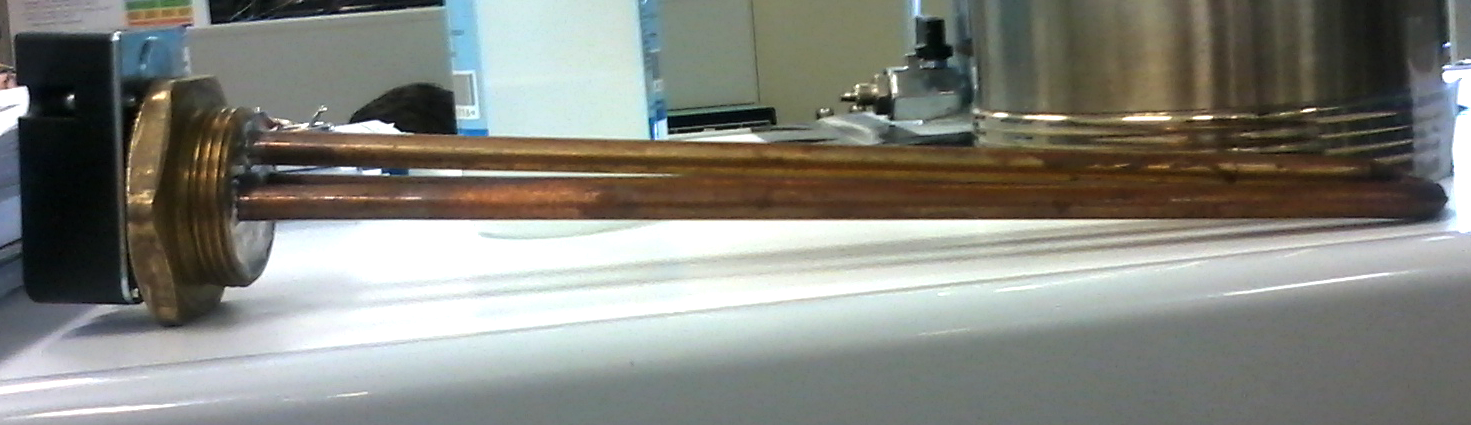
\includegraphics[width=0.9\linewidth]{Figures/4.Chapter/resistencia.png}
\caption{Thermal Resistance used}
\label{fig:res}
\end{figure}

\begin{figure}[h]
\centering
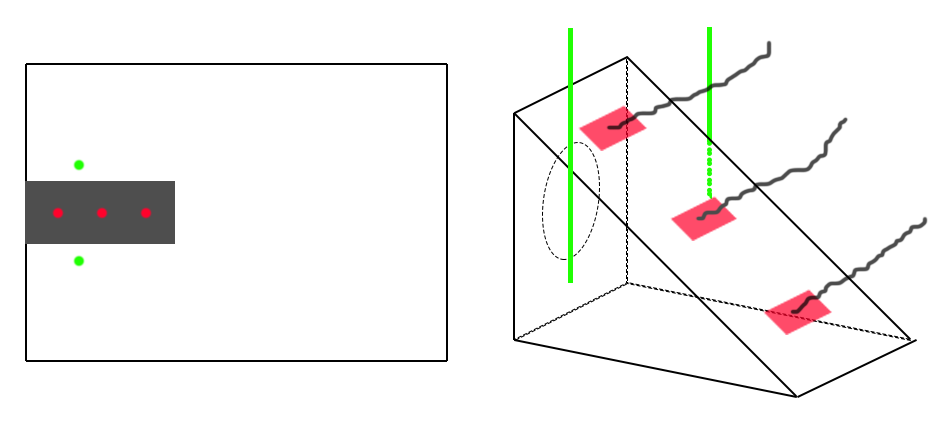
\includegraphics[width=0.9\linewidth]{Figures/4.Chapter/termopares.png}
\caption{Thermocouple placement scheme}
\label{fig:tpar}
\end{figure}

\par The peripherals that the machine needs are: a KS 20-1 PID controller,  that controls the resistance and a DT9828 Data Acquisition Board from Data Translation to connect the thermoucouples to the computer were the data is processed.\\

\par Finally, the insulation consists of a 5mm PENA30FR adhesive, that consists in a sponge with aluminum protection. This can be seen in Figure \ref{fig:isola}. The insulation is used all around the machine and the only hole in it is the hole of the blackbody. \\

\begin{figure}[h]
\centering
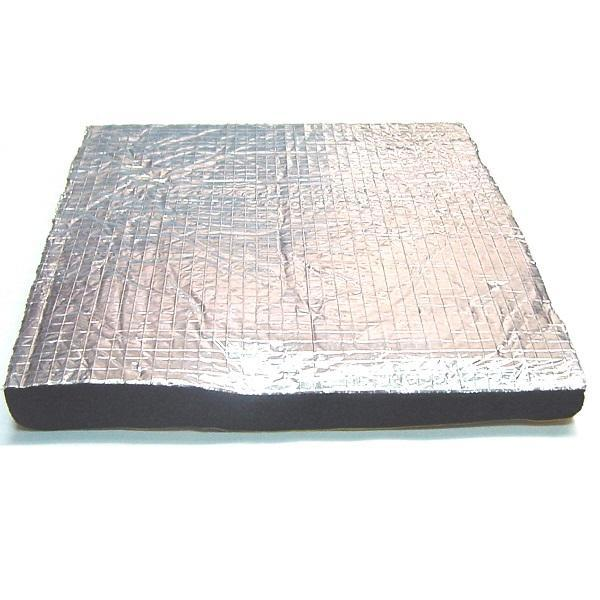
\includegraphics[width=0.5\linewidth]{Figures/4.Chapter/insulation.jpg}
\caption{PENA30FR Adhesive Insulation}
\label{fig:isola}
\end{figure}

\subsection{Building Process}

\par The building process of this machine can be divided in 4 parts:

\begin{itemize}
\item The box: made in stainless steel, this box had to be ordered from a company specialized in metal work. The size of this box is 200x200x320 mm, with 2mm thickness. It already with 2 orifices for both the resistance and the blackbody, but the holes needed to pin the blackbody and sensors to the box had to be made and threaded in the workshop. The thermal insulation was made to fit the box measures. The box is insulated only when both the blackbody and resistance are already installed.
\item The resistance: bought from Mecafil, this resistance was attached to the box with the help of a nut, glued to the back with cold weld. It is also from the resistance hole that all the oil would go in and out. The junction between the nut and the bolt was also reinforced with high temperature silicone, and the screw of the resistance was covered with a Teflon tape to avoid leaks.
\item The blackbody: first a blue print was made and laser cut from a 1mm stainless steel plate, painted with a black matte paint, then bent and finally welded. After the weld, the blackbody had to be re-painted and its insulation reinforced with high temperature silicone. Finally it had to be screwed to its support plate so it could be placed in the box. The end result can be seen in Figure \ref{fig:blkbdy}. This piece was made removable so that new shapes could be made, giving room to the future improvement of the machine. When placed on the machine it is important to put some high temperature silicon to fully prevent any leaks on the machine.
\item The peripherals: starting with the sensors, holes were made on the top of the box so that every sensor could pass through it. The scheme for the holes and the sensors display was already shown in Figure \ref{fig:tpar}. The Data Acquisition Board and the PID controller need to be placed near the box because of the sensor wire length restraint, so a support was made to accommodate everything.
\end{itemize}

\begin{figure}[h]
\centering
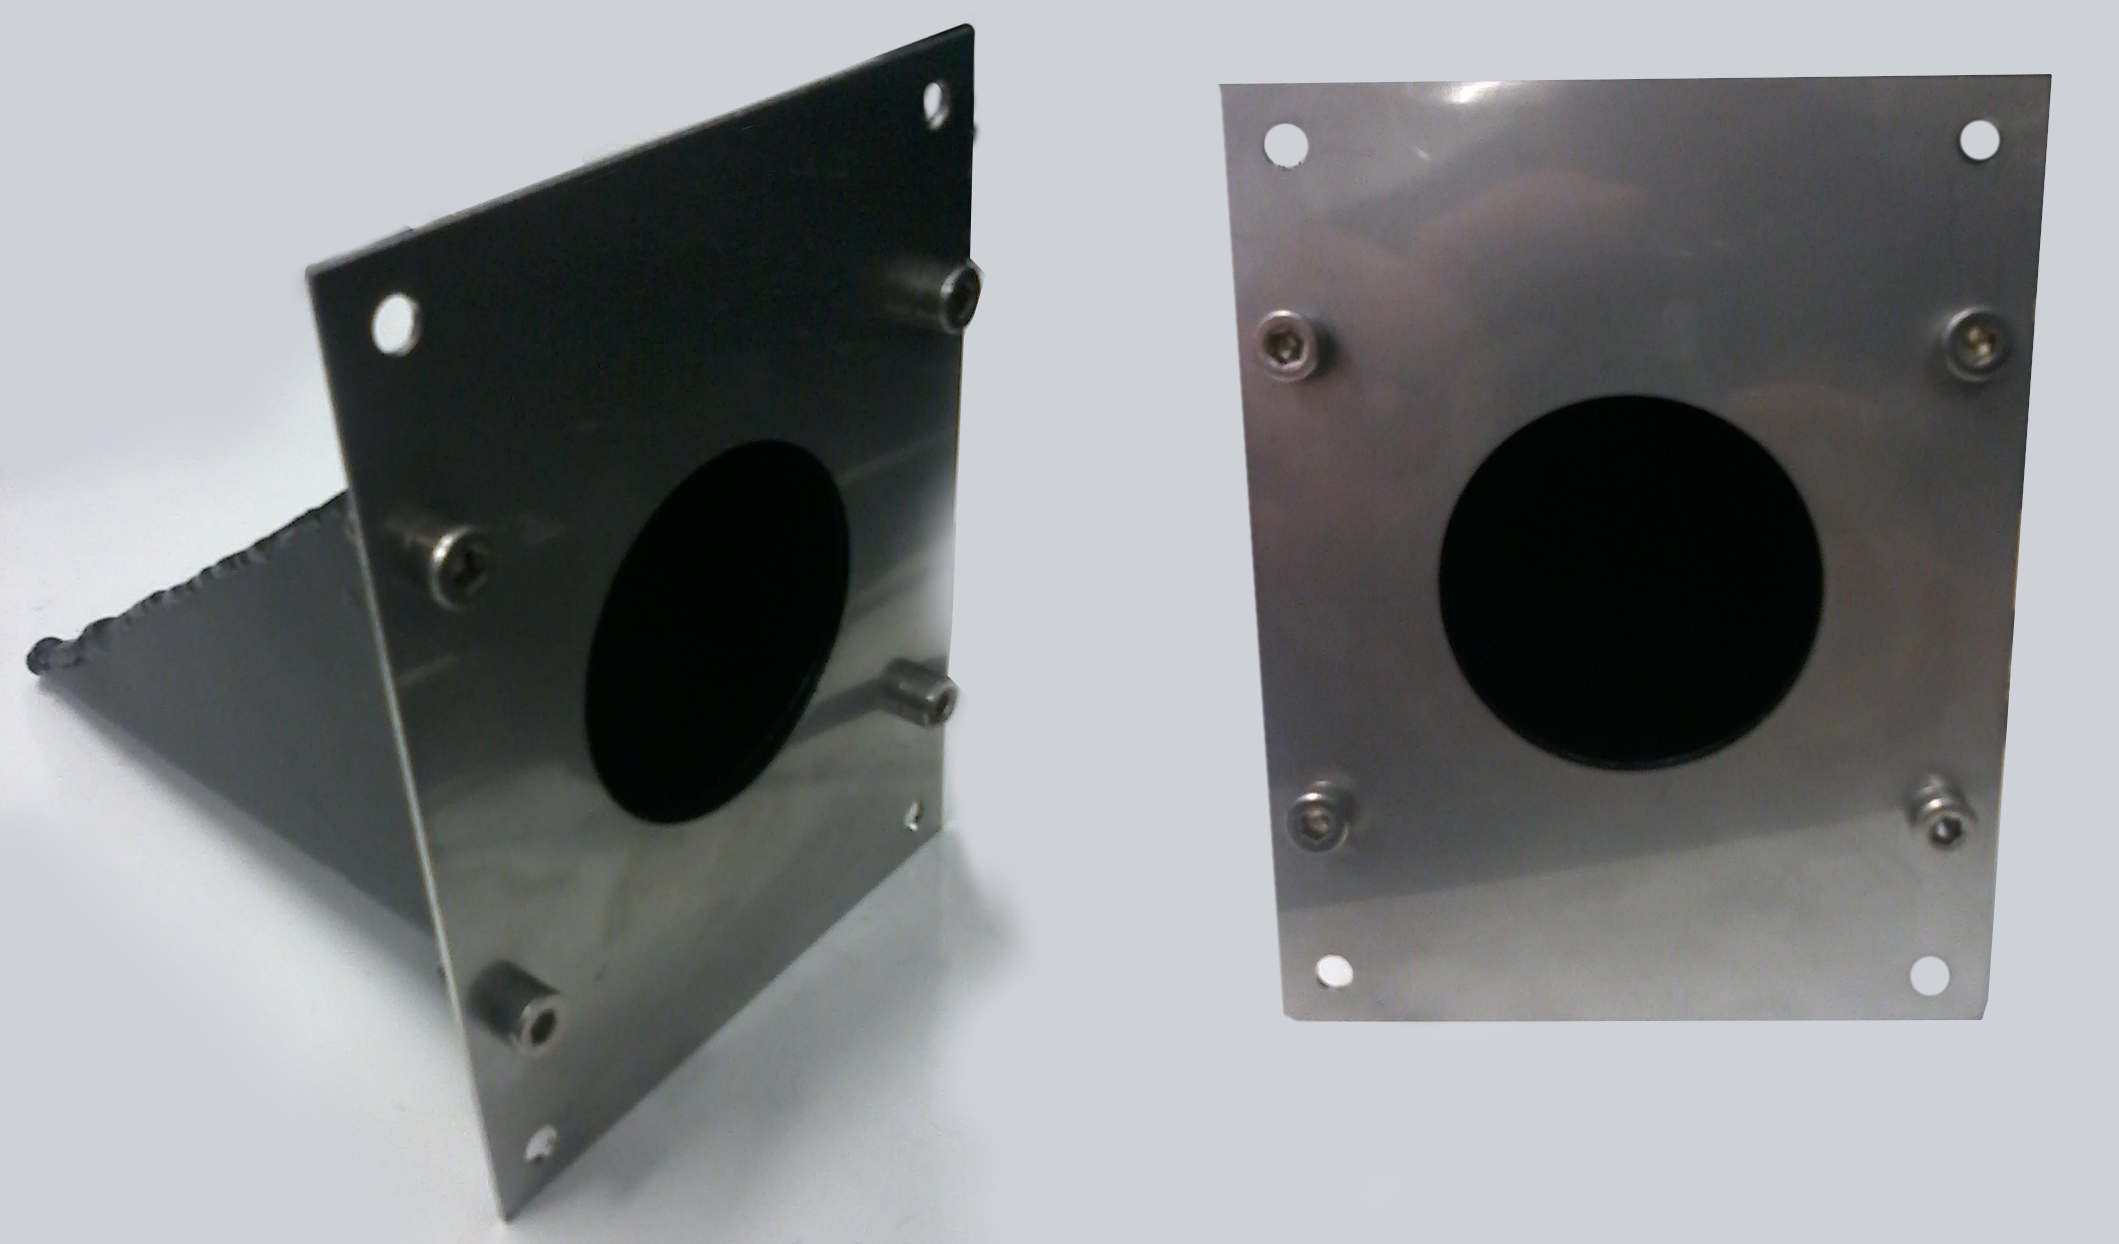
\includegraphics[width=0.7\linewidth]{Figures/4.Chapter/blackbody.png}
\caption{Completed Blackbody}
\label{fig:blkbdy}
\end{figure}

\par The final setup, after all parts were mounted can be seen in Figure \ref{fig:bbcs}. With this setup, it is possible to collect and control temperature values, and correlate them with the camera data, and so it was chosen to perform 2 different calibrations, that will be explained further ahead in this chapter. \\

\begin{figure}[h]
\centering
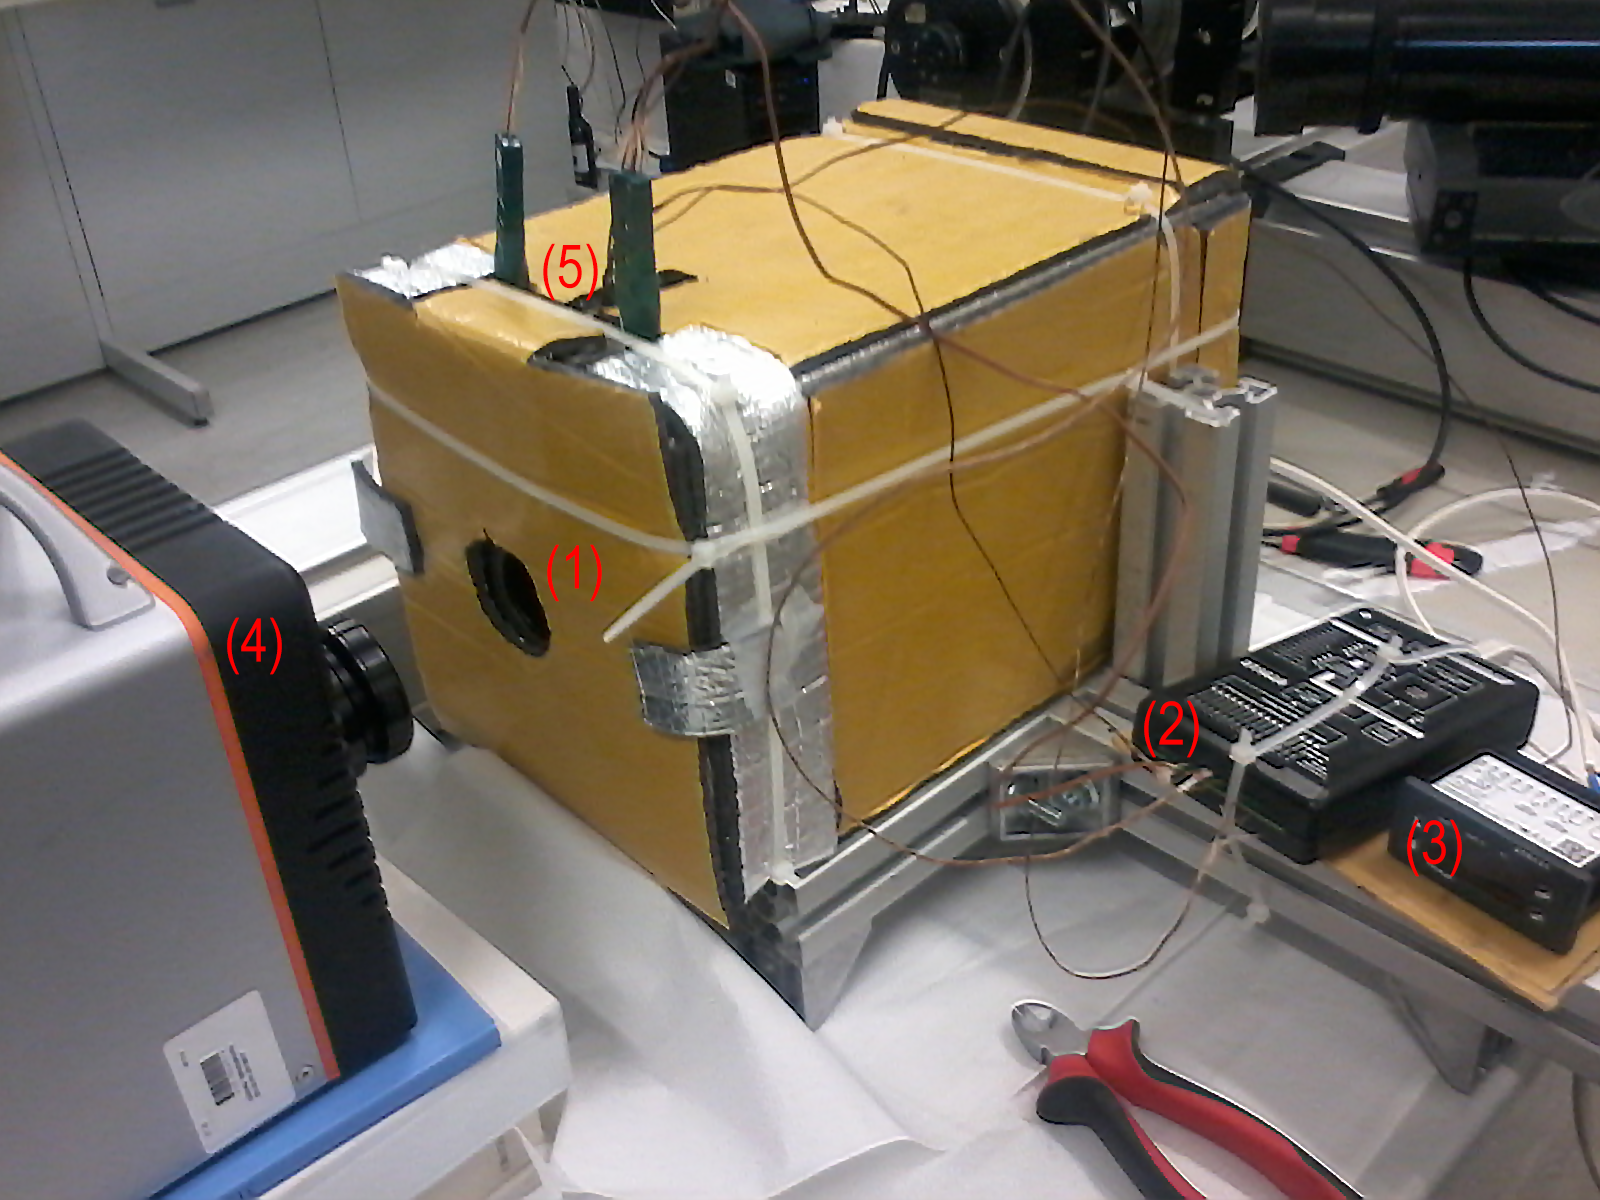
\includegraphics[width=0.7\linewidth]{Figures/4.Chapter/complete.png}
\caption{Completed Blackbody Calibration Source: (1) Blackbody cavity; (2) Data Aquisition Board; (3) PID controller; (4) IR Camera; (5) Thermocouples (one connected to the PID, the others to the Data Aquisition Board)}
\label{fig:bbcs}
\end{figure}

\section{Calibration process}

\par Before the calibration begins there is a set of steps that one needs to take to do it properly:
\begin{itemize}
\item Fill the machine with oil. The oil needs to be taken out of the box after the experiments so it stays clean and it can be stored.
\item Connect the thermocouples to the Data Aquisition Board and to the PID.
\item Turn on the IR Camera and open both its software (Xeneth) and the board software (QuickDAQ).
\item Define an adequate integration time to the desired temperature interval.
\item Do an offset calibration with the camera software.
\end{itemize}

\par It is possible to calibrate the camera in 2 ways now, we can either use the software's calibration feature or use an excel sheet and write the medium ADU value of the cavity region, and then preform the calibration in the post-processing phase. The latter proved to be the best method, but both will be analyzed. \\

\begin{figure}[h]
\centering
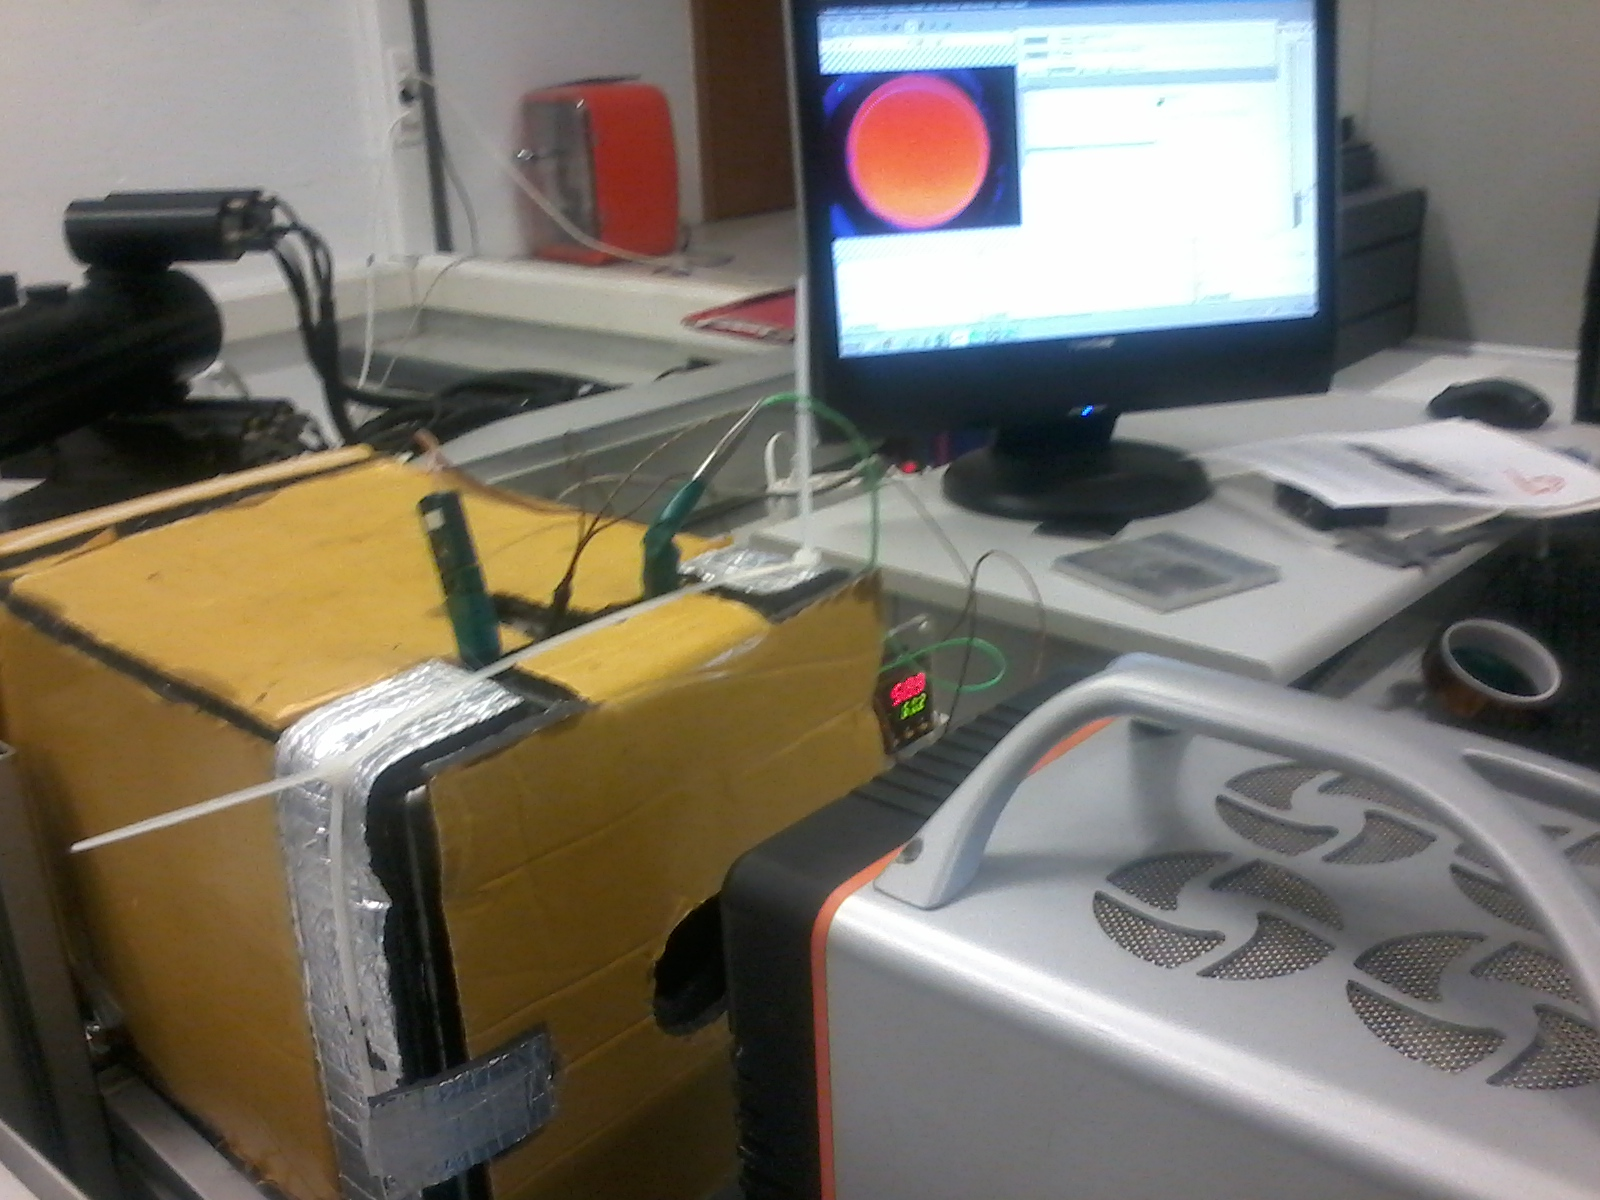
\includegraphics[width=0.55\linewidth]{Figures/4.Chapter/calibinprog.jpg}
\caption{Calibration Instalation in Function}
\label{fig:calibinprog}
\end{figure}

\begin{figure}[h]
\centering
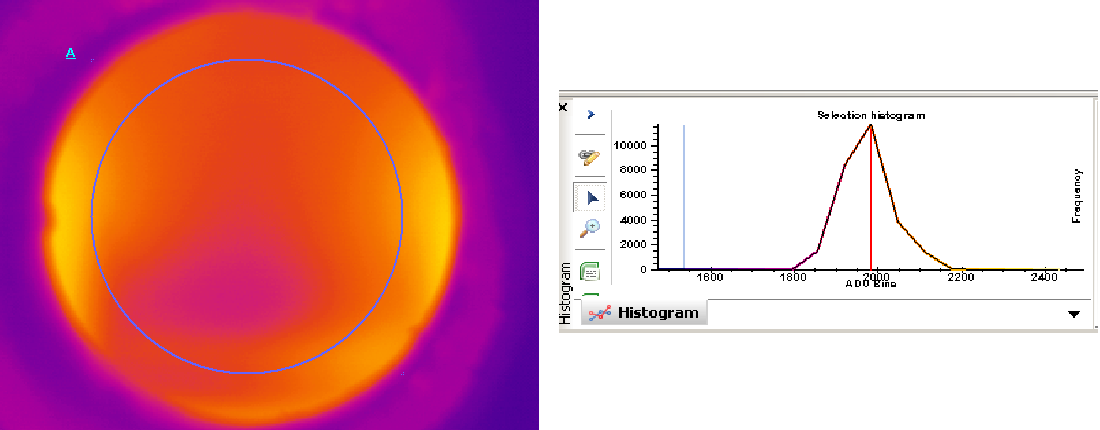
\includegraphics[width=1\linewidth]{Figures/4.Chapter/ex11.png}
\caption{Blackbody thermal image and its respective histogram}
\label{fig:ex1}
\end{figure}

\par During the calibration, the installation looks like Figure \ref{fig:calibinprog}. The first step is to insert the desired temperature (starts with the ambient temperature and then scales in increments of 10ºC/20ºC between measurements) and wait for the temperature to stabilize. In the beginning, what the user will see is shown in Figure \ref{fig:ex1}. It is noticeable here that the edges of the cavity are hotter than the rest. This is due to the fact that the weld that has different thermal properties that the metal sheet, and so it isn't possible to make a calibration right now. \\

\par This may be a problem, but the PID controller solves it. The following is a simplified description of how the PID controller works to give context. A temperature is inserted in the PID controller, then compares it with the thermocouple's temperature and if the thermocouple's temperature is below the desired temperature it turns on the resistance. Just before the oil is at the desired temperature, it turns off the resistance in order to account for the response delay. When the resistance is off the temperature cools and when it reaches a certain temperature bellow the desired temperature, it turns on the resistance again. This cycle is repeated to keep the system at the desired temperature. \\

\begin{figure}[h]
\centering
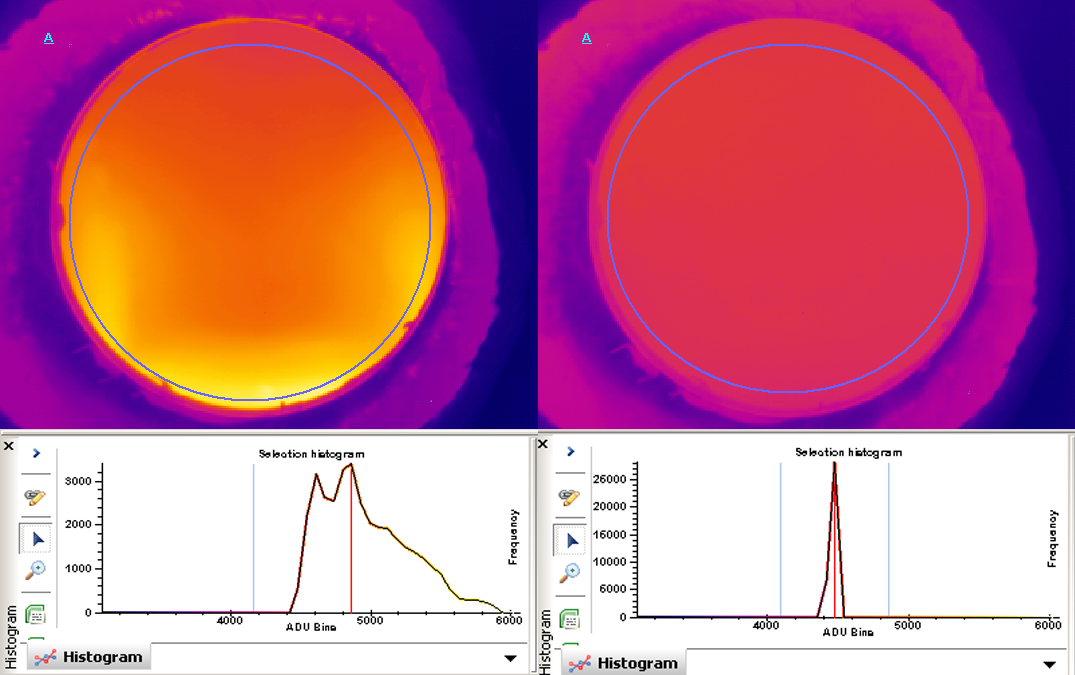
\includegraphics[width=0.9\linewidth]{Figures/4.Chapter/ex2.png}
\caption{Xeneth's software - Temperature Calibration (Plank)}
\label{fig:ex2}
\end{figure}

\par With this context given, it is possible now to explain how can we get an uniform temperature on the cavity. When the resistance is off, because of the thermal inertia of the oil and the good insulation of the machine we can get a more uniform temperature, as it stabilizes while cooling down. This can be clearly seen in Figure \ref{fig:ex2}. In the left we have the temperature map once we reach the desired temperature for the first time. After a few minutes, it is possible to see what's in the right. Please pay attention to the histograms for they show exactly what is desired for the ideal temperature measurement: in the left we can see a wider range of values, and in the right there is clearly a peak. This means that on the circle marked as A the temperature got much more uniform and it's now possible to take a measurement. \\

\par To see what temperature corresponds to the averaged ADU value, an average of the surface thermocouple read temperatures in time was taken, with the help of the software QuickDAQ, which allows to take a data sample for a fixed amount of time. This is used to make the average between all the surface thermocouples connected to the board and the value shown in the PID. This final average is then the input for the software calibration or saved with the ADU in an excel for the second method. \\

\subsection{Software Calibration}

\par The Xenics' software has a camera calibration wizard (in which the offset calibration feature is included) that automatically correlates the ADU's with temperature measured. The feature described is called "Temperature Calibration (Plank)" and can be seen in Figure \ref{fig:plankcalib}. In the shown interface, the user can input the temperature measured by the thermocouples in the field (a), and then add the read value with button (b). It will then add a point, to the table at the left and draw in on a graph bellow. This point has the given temperature, and the ADU measured with a spatial average of a small rectangular area in the center of the image. \\

\begin{figure}[h]
\centering
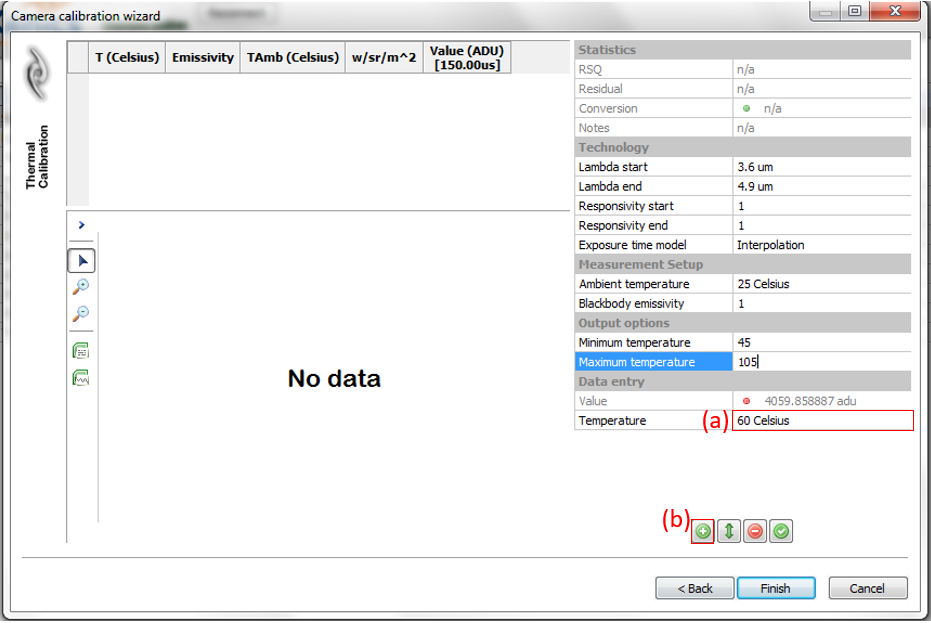
\includegraphics[width=0.7\linewidth]{Figures/4.Chapter/plankcalib.png}
\caption{Xeneth's software - Temperature Calibration (Plank)}
\label{fig:plankcalib}
\end{figure}

\par In the first calibration, this method was tried but because the temperature and respective measured ADU are shown it didn't invalidate the possibility to use them in the second method. In this attempt the integration time of 450 was used. The final table and graphic can be seen in Figure \ref{fig:calib}. On the table labeled as (a) it's possible to see 5 columns. The first column and the last represent the read values of temperature and ADU. The second and third column represent the ambient temperature and emissivity which are actually irrelevant for this case because we are assuming we have a perfect blackbody, so the ambient temperature won't be used in this calibration. The fourth column is a variable, which varies with the input temperature, that the software uses to convert, together with the other inputs, the temperature, in what the software calls "Soaled Radiance", represented in the x axys of graph (b) in Figure \ref{fig:calib}. This variable is not explained in the manual, nor its relation with the temperature. This was one of the disadvantages of this method mainly because the software creates the "Soaled Radiance" value out of it, and it is supposed to mantain a proportional relation with the ADU's so the calibration is described by a line. But as it is noticeable in the graph, the values didn't follow the line that closely, which caused a deviation significant enough to make this method unusable. \\

\par Having this variable and the "Soaled Radiance" unexplained, the only option was to take these values and use them in the other method. Another reason is that this method does a linear correlation. This may only be a vague assumption or a rough approximation, and because even if the origin of these variables was known, there would be no way to validate that linear relation. \\

\par In the end, the software creates a calibration convertion that can be selected when it is opened and used to take the data directly in Celsius. This calibration file can only be used for the specified integration time. In Figure \ref{fig:calib} it's possible to see how the software approximates linearly (green line) the measured points (red line). Because this calibration didn't match the experimental values as close as desired, when the newly created calibration pack was tested it didn't work properly, so the second type of calibration was made. \\

\begin{figure}[h]
\centering
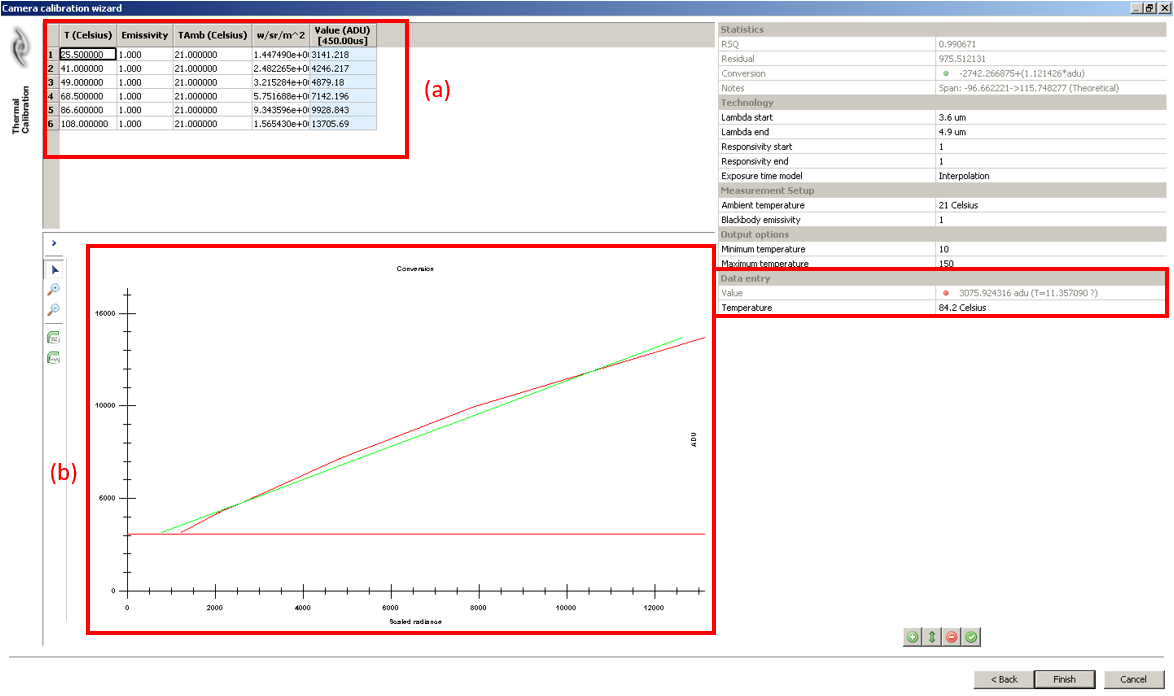
\includegraphics[width=0.7\linewidth]{Figures/4.Chapter/calibracao.png}
\caption{Complete Temperature Calibration (Plank)}
\label{fig:calib}
\end{figure}

\subsection{Proposed Calibration}

\par In this method the calibration results are taken directly from the software, without using the software's Calibration Wizard. They're saved in an Microsoft Excel sheet along with the average temperature read by the thermocouples. With this method the results have to be taken raw from the software and then process them with the matlab code that was made just for this purpose. A whole explanation of the process will be given in the next section, leaving in this section a general outline of the proposed method.\\

\par The process of data aquisition for the calibration is similar to the previous calibration. The main difference in this method is the absence of the Calibration Wizard. Instead, the Selection Panel (described in \ref{software}) is used to gather the average measured ADU of a circular area, similar to what can be seen in Figure \ref{fig:ex2}. There are several advantages in this method, one being that it was now possible to adjust the temperature range (the Calibration Wizard didn't allow it), and better understand when the image saturates. Another advantage is the fact that it is possible to change integration time. \\

\par In Microsoft Excel, the measured temperatures are converted into the radiated energy using equation \ref{eq:6} (and considering the object perfectly black) and plotted against the ADU. Then Microsoft Excel's trending line function is used to extract a polynomial curve that will best approximate the data gathered in the experiments. The second and third degree polynomial approximations were compared, but in the end the third degree polynomial. This option took longer to process but the end result was significantly closer to the experimental results. \\

\par With the extracted curve a MATLAB code was made to calibrate the videos. The raw data video data (in ADU) matrix is the input of this function. This matrix has the value for every pixel in every frame, and point by point is solving the following equation:

\begin{equation}
A \times W_{tot}^3 + B \times W_{tot}^2 + C \times W_{tot} + D = ADU_{pixel}
\end{equation}

in which A,B,C and D are the coefficients of the calculated polynomial curve, $ADU_{pixel}$ is the pixel ADU value and $W_{tot}$ is the wanted radiated energy. Using this radiated energy value, the pixel temperature is calculated using equation \ref{eq:7}. The end result is a matrix with all the temperatures.

\subsection{Calibration Process Details}

\par One important fact about the designed calibration procedure is that it took a whole day to complete. This is due to the fact that there was no refrigeration system and the liquid had to cool at room temperature. It would also have some problems at high temperatures with leaks. This took some time to address and caused that the calibration process couldn't often be repeated. \\

\par Two calibrations were made during this work. The first was made using the software at the fixed integration time of 450us. The second was made using the proposed method for the integration times of 450us and 200us. With the integration time of 450us the image would saturate at around 108ºC, so the correspondent results weren't suited for our experiment. \\

\par The results of the calibration can be seen in Table \ref{tab:calibration}. Because the results were taken for both calibrations at $it=450us$ we can use them to prove the method's consistency. The comparison can be seen in Figure \ref{fig:calibplot}.  \\

\begin{table}[h]
\centering
\caption{Calibration Results}
\label{tab:calibration}
\begin{tabular}{ccccccccc}
\toprule
\multicolumn{3}{c}{Calibration 1}       &  & \multicolumn{5}{c}{Calibration 2}                                    \\ 
\cmidrule[0.4pt](r{0.125em}){1-3}%
\cmidrule[0.4pt](r{0.125em}){5-9}%
         & \multicolumn{2}{c}{it=450us} &  &        & \multicolumn{2}{c}{it=450us} & \multicolumn{2}{c}{it=200us} \\
\cmidrule[0.4pt](r{0.125em}){2-3}%
\cmidrule[0.4pt](r{0.125em}){6-7}%
\cmidrule[0.4pt](r{0.125em}){8-9}%
T(ºC)  & ADU         & $W_{tot}(W/m^2)$      &  & T(ºC)& ADU         & $W_{tot}(W/m^2)$      & ADU         & $W_{tot}(W/m^2)$      \\
\cmidrule[0.4pt](r{0.125em}){1-3}%
\cmidrule[0.4pt](r{0.125em}){5-9}%
25.5     & 3141        & 450.1533       &  & 25.46  & 3200        & 449.912        & 1645        & 449.912        \\
41       & 4246        & 551.1904       &  & 34.5   & 3794        & 506.9481       & 1900        & 506.9481       \\
49       & 4879        & 609.5461       &  & 44.28  & 4666        & 574.5844       & 2285        & 574.5844       \\
68.5     & 7142        & 771.1625       &  & 62.27  & 6287        & 716.4103       & 3021        & 716.4103       \\
86.6     & 9928        & 948.1167       &  & 75.76  & 8270        & 838.8605       & 3890        & 838.8605       \\
108      & SAT         & SAT            &  & 84.33  & 9827        & 924.4022       & 4596        & 924.4022       \\
         &             &                &  & 94.54  & 12094       & 1034.669       & 5586        & 1034.669       \\
         &             &                &  & 103.67 & 14078       & 1141.372       & 6690        & 1141.372       \\
         &             &                &  & 114.39 & SAT         & SAT            & 8139        & 1276.958       \\
         &             &                &  & 125.74 & SAT         & SAT            & 9885        & 1433.317     \\ \bottomrule
\end{tabular}
\end{table}

\begin{figure}[h]
\centering
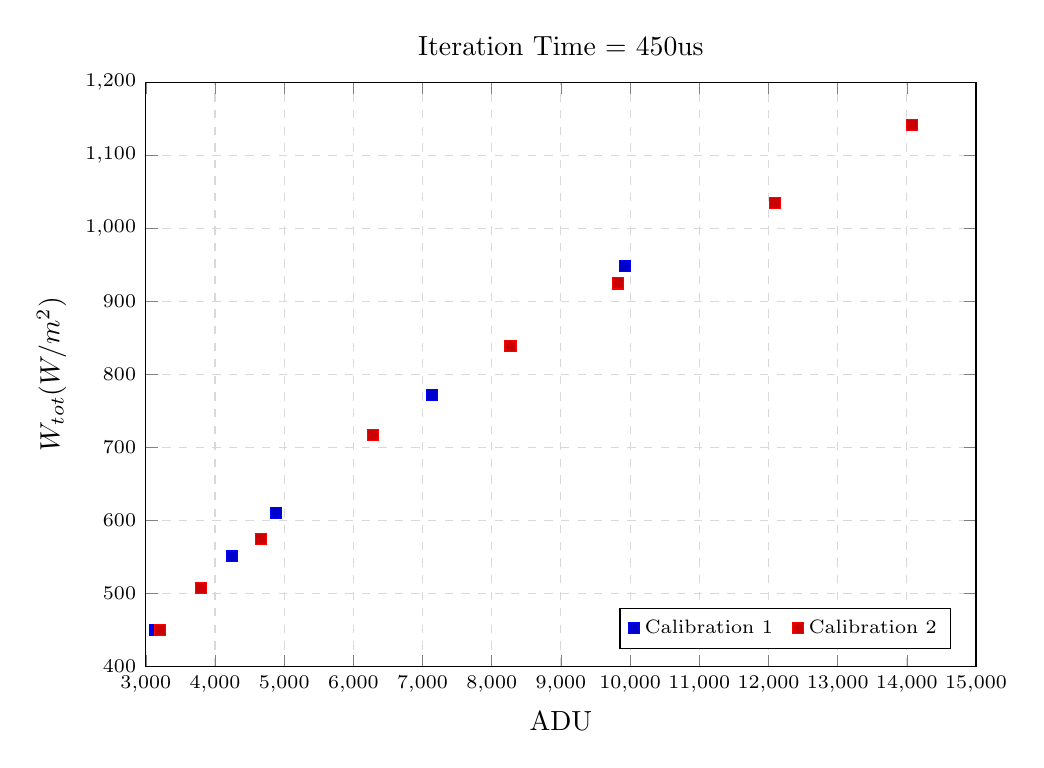
\begin{tikzpicture}
\begin{axis}[
	title = {Iteration Time = 450us},
    tick label style={font=\scriptsize},
    legend style={font=\scriptsize,/tikz/column 2/.style={column sep=5pt},},
    legend columns=2,
    legend cell align=left,
	legend pos =south east,
    grid=major, % Display a grid
    grid style={dashed,gray!30}, % Set the style
    xlabel={ADU},
    ylabel={$W_{tot} (W/m^2)$}, 
    ymin = 400, ymax = 1200,
    %ytick={300,325,350,375,400,425,450,475,500,525},
    %yticklabels={300,325,350,375,400,425,450,475,500,525},
    xmin = 3000, xmax = 15000,
    xtick={0,1000,...,15000},
    xticklabel style={
        /pgf/number format/fixed,
        /pgf/number format/precision=5},
	scaled x ticks=false,
    width=\textwidth, height=9cm,
    %legend entries={Experimental,Computational, $264 W/m^{2}$,$807 W/m^{2}$,$2031 W/m^{2}$,$3636 W/m^{2}$}
    ]

% \addlegendimage{only marks, mark=square*,black}
% \addlegendimage{only marks, mark=x      ,black}
% \addlegendimage{only marks, mark=*      ,blue}
% \addlegendimage{only marks, mark=*      ,red}
% \addlegendimage{only marks, mark=*      ,brown}
% \addlegendimage{only marks, mark=*      ,black}


%-------------------------------------------------------------
%Experimental ------------------------------------------------
%-------------------------------------------------------------

\addplot+[only marks,mark=square*,blue] % 264 experimental
coordinates {(	3141	,	450.1532612	)
(	4246	,	551.1904079	)
(	4879	,	609.5460842	)
(	7142	,	771.1624794	)
(	9928	,	948.1166888	)
};
\addplot+[only marks,mark=square*,red]
coordinates{(	3200	,	449.9120215	)
(	3794	,	506.9481463	)
(	4666	,	574.5844207	)
(	6287	,	716.4103256	)
(	8270	,	838.8604805	)
(	9827	,	924.4022127	)
(	12094	,	1034.669156	)
(	14078	,	1141.371929	)};
\legend{Calibration 1, Calibration 2}

\end{axis}
\end{tikzpicture}
\caption{Comparison of the two calibrations at it=450us}
\label{fig:calibplot}
\end{figure}

\par Next, the $it=200us$ data has to be plotted, and a trending line calculated. The data with the correspondent trending line can be seen in Figure \ref{fig:calibcurve}. The equation that is represented in the plot is the one used in the calibration code. \\

\begin{figure}[h]
\centering
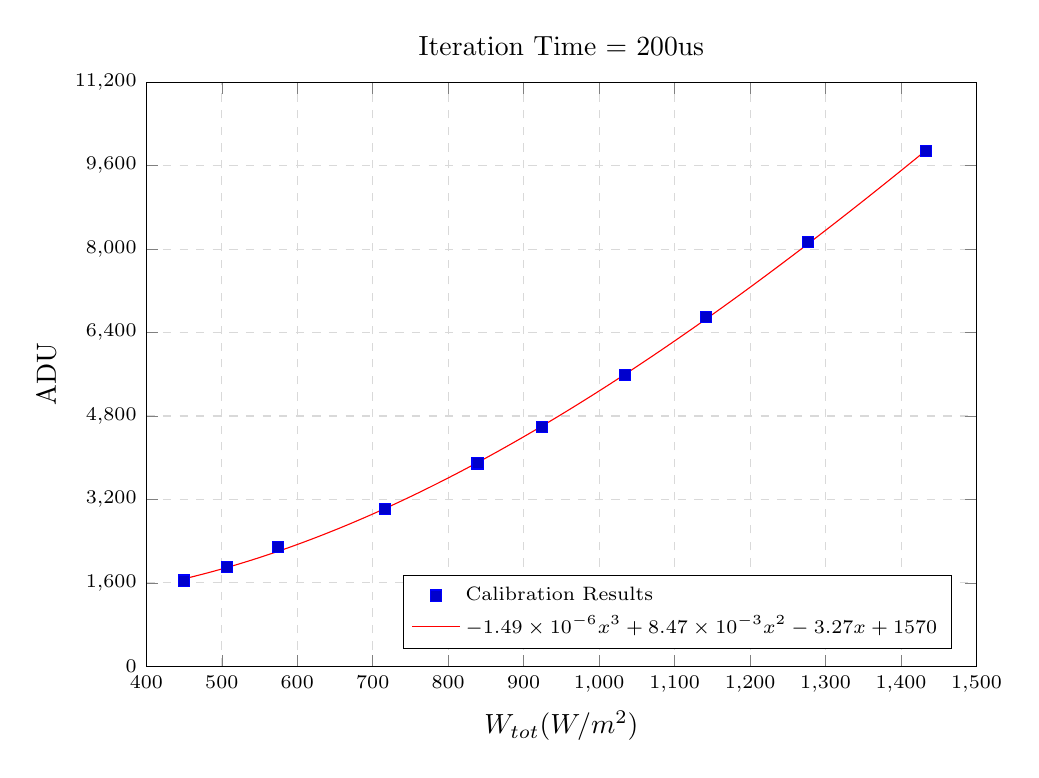
\begin{tikzpicture}
\begin{axis}[
	title = {Iteration Time = 200us},
    tick label style={font=\scriptsize},
    legend style={font=\scriptsize,/tikz/column 2/.style={column sep=5pt},},
    %legend columns=2,
    legend cell align=left,
	legend pos =south east,
    grid=major, % Display a grid
    grid style={dashed,gray!30}, % Set the style
    xlabel={$W_{tot} (W/m^2)$},
    ylabel={ADU}, 
    ymin = 0, ymax = 11200,
    %ytick={300,325,350,375,400,425,450,475,500,525},
    %yticklabels={300,325,350,375,400,425,450,475,500,525},
    xmin = 400, xmax = 1500,
    ytick={0,1600,...,11200},
    yticklabel style={
        /pgf/number format/fixed,
        /pgf/number format/precision=5},
	scaled y ticks=false,
    width=\textwidth, height=9cm,
    ]
\addplot+[only marks,mark=square*,blue]
coordinates {(	449.9120215	,	1645	)
(	506.9481463	,	1900	)
(	574.5844207	,	2285	)
(	716.4103256	,	3021	)
(	838.8604805	,	3890	)
(	924.4022127	,	4596	)
(	1034.669156	,	5586	)
(	1141.371929	,	6690	)
(	1276.958202	,	8139	)
(	1433.317083	,	9885	)
};
\addlegendentry{Calibration Results}
\addplot[
    domain=450:1430, 
    samples=100, 
    color=red,
]{0.00847*x^2 - 0.00000149*x^3 - 3.27*x + 1570};
\addlegendentry{$-1.49\times 10^{-6}x^3 + 8.47\times 10^{-3}x^2 - 3.27x + 1570$}
\end{axis}
\end{tikzpicture}
\caption{Comparison of the two calibrations at it=450us}
\label{fig:calibcurve}
\end{figure}

\par The generated code is used to transform every video from ADU values to Celsius, and works only for the selected integration time. The code can also be easily adapted to the integration time of 450us. This code can be seen in Appendix \ref{ap:a}. \\

\clearpage

\section{Data Processing Methods}
\par The collected images, without any sort of treatment, have some random noise and unwanted patterns of noise. While the noise source is usually small differences in sensitivity or calibration of the sensors, the patterned noise has it's origin mainly on the software processing. A temperature difference is always noticeable inside the region of interest. This cannot be solved so, to accurately evaluate the results, a background remove has to be performed. This also helps removing some background noise. \\

\par To be treated, the video needs to be imported to avi format, in an 8 bit, grey scale format. In MATLAB, the video is divided into frames and the grey scale value transformed to temperature, considering the temperature or ADU scale it was imported with. After this, the calibration is applied and finally the filters. In the end, the results are extracted as a MATLAB file with all values and a txt with the results from the center to the radius of the droplet with a plot option.

\subsection{Patterned Noise}

\par The origin of this type of noise was detected in the software's zoom function. It can result in significant errors. At constant temperature the results showed that the  difference between pixels side by side was 1ºC. To remove this, a filter was made that would add and subtract 0.5ºC alternately. The generated pattern and the effect of the filter can be seen in Figure \ref{fig:chess}.

\begin{figure}[h]
\centering
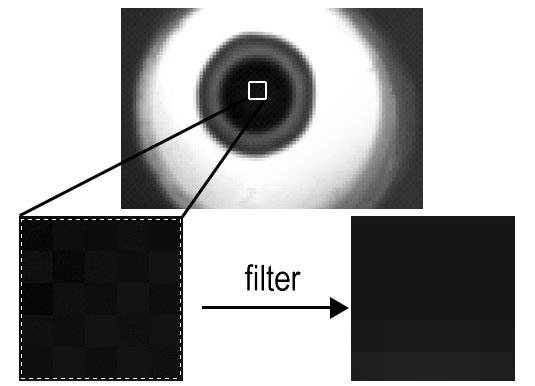
\includegraphics[width=0.5\linewidth]{Figures/4.Chapter/chess2.png}\\
\subfigure{
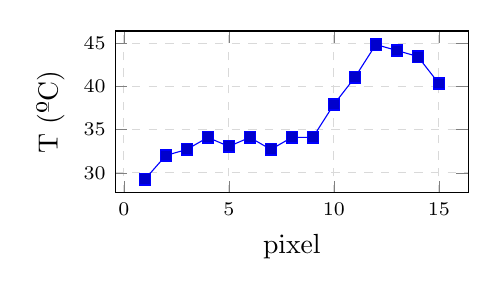
\begin{tikzpicture}
\begin{axis}[
	width=0.5\linewidth,
    height=0.3\linewidth,
	%title = {Unprocessed Results},
    tick label style={font=\scriptsize},
    legend style={font=\scriptsize,/tikz/column 2/.style={column sep=5pt},},
    %legend columns=2,
    legend cell align=left,
	legend pos =south east,
    grid=major, % Display a grid
    grid style={dashed,gray!30}, % Set the style
    xlabel={pixel},
    ylabel={T (ºC)}, 
    %ymin = 0, ymax = 11200,
    %ytick={300,325,350,375,400,425,450,475,500,525},
    %yticklabels={300,325,350,375,400,425,450,475,500,525},
    %xmin = 400, xmax = 1500,
    %ytick={0,1600,...,11200},
    %yticklabel style={
    %    /pgf/number format/fixed,
    %    /pgf/number format/precision=5},
	%scaled y ticks=false,
    ]
\addplot+[mark=square*,blue]
coordinates {(	1	,	29.23	)
(	2	,	32	)
(	3	,	32.7	)
(	4	,	34.09	)
(	5	,	33.05	)
(	6	,	34.09	)
(	7	,	32.7	)
(	8	,	34.09	)
(	9	,	34.09	)
(	10	,	37.9	)
(	11	,	41.03	)
(	12	,	44.84	)
(	13	,	44.15	)
(	14	,	43.45	)
(	15	,	40.33	)
};
%\addlegendentry{}
\end{axis}
\end{tikzpicture}
}%
\subfigure{
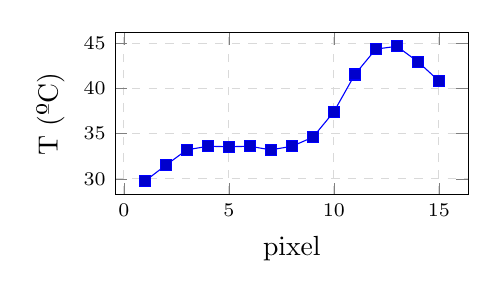
\begin{tikzpicture}
\begin{axis}[
	width=0.5\linewidth,
    height=0.3\linewidth,
	%title = {Processed Results},
    tick label style={font=\scriptsize},
    legend style={font=\scriptsize,/tikz/column 2/.style={column sep=5pt},},
    %legend columns=2,
    legend cell align=left,
	legend pos =south east,
    grid=major, % Display a grid
    grid style={dashed,gray!30}, % Set the style
    xlabel={pixel},
    ylabel={T (ºC)}, 
    %ymin = 0, ymax = 11200,
    %ytick={300,325,350,375,400,425,450,475,500,525},
    %yticklabels={300,325,350,375,400,425,450,475,500,525},
    %xmin = 400, xmax = 1500,
    %ytick={0,1600,...,11200},
    %yticklabel style={
    %    /pgf/number format/fixed,
    %    /pgf/number format/precision=5},
	%scaled y ticks=false,
    ]
\addplot+[mark=square*,blue]
coordinates {(	1	,	29.73	)
(	2	,	31.5	)
(	3	,	33.2	)
(	4	,	33.59	)
(	5	,	33.55	)
(	6	,	33.59	)
(	7	,	33.2	)
(	8	,	33.59	)
(	9	,	34.59	)
(	10	,	37.4	)
(	11	,	41.53	)
(	12	,	44.34	)
(	13	,	44.65	)
(	14	,	42.95	)
(	15	,	40.83	)
};
%\addlegendentry{}
\end{axis}
\end{tikzpicture}
}
\caption{Chess pattern example}
\label{fig:chess}
\end{figure}


\subsection{Median Filter}

\par This filter has the potential to remove random bad pixels noise from the picture. This filter is a MATLAB function that outputs the median of a 3-by-3 neighborhood of the input pixel. With this simple filter the image can be greatly improved as shown in Figure \ref{fig:median}. On the right there's the image without the filter and on the left the treated image.

\begin{figure}[h]
\centering
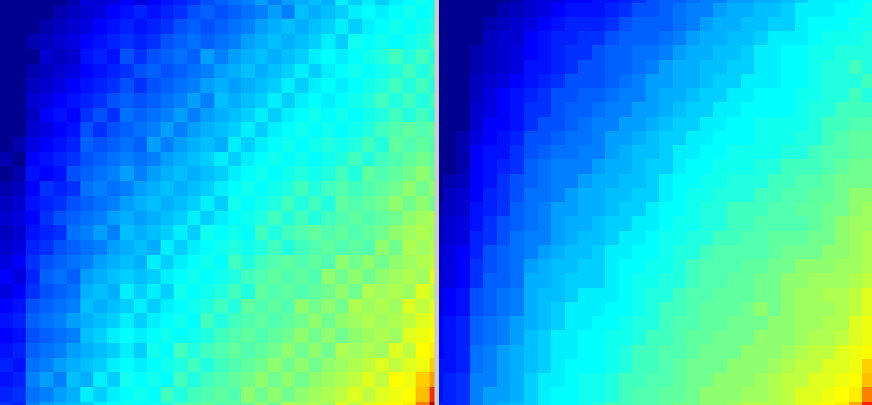
\includegraphics[width=0.6\linewidth]{Figures/4.Chapter/median.png}
\caption{Median filter effect}
\label{fig:median}
\end{figure}

\subsection{Background Filter}
\par The background filter serves the function of eliminating any problems related with the optics of the camera and to equalize the temperature field. Two different ways to do it were thought. Two MATLAB codes were made and tested. The first one is the simple way and is shown in Equation \ref{eq:bkg}. The variable $vid$ is the matrix with the temperature value for every pixel in every frame, $avTemp$ is the average temperature in the center of the hole and $t_n$ is the number of the analyzed frame.
\begin{equation}\label{eq:bkg}
vid^{*}(x,y,t_n)=vid(x,y,t_n)-vid(x,y,1)+avTemp
\end{equation}
\par The second one is a weighted background removal and we can see it in Equation \ref{eq:pbkg}. The variables bear the same meaning, but has to be done for each pixel ($x_p,y_p$). Only the code for the latter can be seen in Appendix \ref{ap:b} as the code is similar in both cases. 
\begin{equation}\label{eq:pbkg}
vid^{*}(x_p,y_p,t_n)=\frac{vid(x_p,y_p,t_n)-vid(x_p,y_p,1)}{vid(x_p,y_p,1)}avTemp+avTemp
\end{equation}
\begin{figure}[h]
\centering
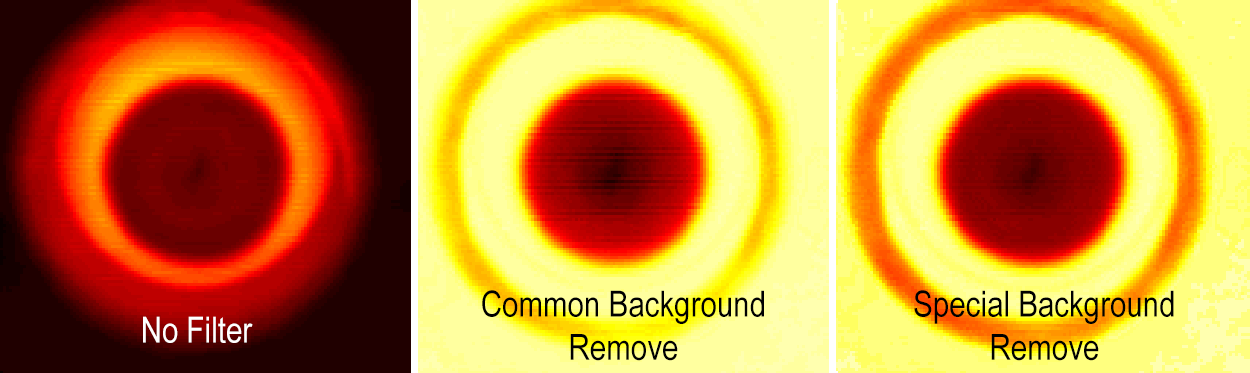
\includegraphics[width=0.8\linewidth]{Figures/4.Chapter/bkg.png}
\caption{Background filter effect}
\label{fig:bkg}
\end{figure}

\subsection{Heat Flux computation}

\par To evaluate and compare the heat removal capacity of the system it is very important to compute the heat flux and cooling effectiveness, mentioned in Section \ref{sec:heat}. This was also made with the help of a MATLAB code, that can be seen in Appendix \ref{ap:c} and \ref{ap:d}.\\
\par Starting with the computation of the
